% IEEE Transactions on Medical Imaging — MIC v5
% Changes from v4:
%  - Expanded acronyms throughout (ANS, FSE, DICOM, HTJ2K, PACS, RLE, CR, XR,
%    EBCOT, MED, CALIC, FLIF, tANS, rANS, LZ77, SIMD, AVX2, CGO, BMI2, etc.)
%  - Added plain-language SE-accessibility sentences in abstract and method
%  - Added numeric residual example in introduction
%  - Added byte-splitting concrete example
%  - Clarified 65,535 vs 65,536 (overflow delimiter reserves one code)
%  - Clarified 4,096 vs 4,095 (now consistent: 4,096 throughout)
%  - Added residual-code table and decode pseudocode in Section III.B
%  - Defined midCount protocol fully; added RLE encoding example
%  - Added "FSE in one paragraph" overview in Section III.D
%  - Defined symbolLen / symbolDensity precisely in Section III.E
%  - Explained why Huffman backend is slower in Section III.F
%  - Added four-state bitstream format description in Section IV
%  - Improved magic-header explanation in Section IV.B
%  - Clarified Go vs C compiler flags; corrected CPU topology in Section V.D
%  - Added variant comparison table in Section V.D
%  - Added PICS definition earlier (Section V.D)
%  - Added "Practitioner takeaway" paragraph in Section VI
%  - Softened pre-results JPEG-LS claim in Related Work
%  - Reduced repetition of JPEG-LS, browser-decoder, and speedup claims
%  - Fixed em-dash overuse throughout
%  - Fixed "18x less" -> "18x fewer source lines"; "within 1%" -> "within 1% relative to"
%  - Browser claim now hedged with "at the time of writing"
%  - XA1 footnote rephrased (no longer claims measurement noise)
% Compile: pdflatex -> bibtex -> pdflatex -> pdflatex
\documentclass[journal]{IEEEtran}

% ---- Math / fonts ----
\usepackage{amsmath}
\usepackage{amssymb}
\usepackage{amsthm}

% ---- Graphics / tables ----
\usepackage{graphicx}
\usepackage{booktabs}
\usepackage{array}
\usepackage{multirow}

% ---- Utilities ----
\usepackage{xcolor}
\usepackage{url}
\usepackage{hyperref}
\usepackage{microtype}
\usepackage{listings}
\usepackage{algorithm}
\usepackage{algpseudocode}
\usepackage{caption}
\usepackage{subcaption}
\usepackage{cite}

\hypersetup{
  colorlinks=true,
  linkcolor=blue!70!black,
  citecolor=green!50!black,
  urlcolor=blue!70!black,
}

\lstset{
  basicstyle=\ttfamily\small,
  breaklines=true,
  columns=fullflexible,
}

% --------------------------------------------------
\title{A 16-Bit-Native Entropy Coding Pipeline for\\
       Lossless Medical Image Compression}

\author{Kuldeep~Singh%
\thanks{K.\ Singh is with Innovaccer Inc.
E-mail: kuldeep.singh@innovaccer.com.
Code: \url{https://github.com/pappuks/medical-image-codec}.}%
}


% --------------------------------------------------

\begin{document}
\maketitle

% ============================================================
\begin{abstract}
Lossless compression remains important in medical imaging because archival
storage, transmission, and diagnostic workflows often require exact
reconstruction of high-bit-depth pixel data. Many medical images are stored at
10--16 bits per sample, yet most practical compression software remains
optimized for byte-oriented processing or small symbol alphabets. This paper
studies a lossless compression pipeline designed to operate natively on
predicted 16-bit residuals.

We present MIC, a codec consisting of three stages: spatial prediction, 16-bit
run-length encoding, and large-alphabet table-based asymmetric numeral
systems (ANS) coding. In contrast to codecs that split 16-bit pixels into
byte pairs before entropy coding, MIC treats each predicted residual as a
single 16-bit symbol, allowing the entropy model to capture correlations
between the high and low byte directly. The implementation extends
Finite State Entropy (FSE), a table-driven ANS variant, to support large
active symbol sets arising in medical image residual streams and includes a
multi-state interleaved decoder that increases instruction-level parallelism
(ILP) during decompression. The design is motivated by the observation that,
after simple spatial prediction, many medical images produce residual
distributions sharply concentrated near zero with frequently repeated 16-bit
residual values.

Evaluation on 21 de-identified DICOM images spanning nine modalities shows the
16-bit-native pipeline improves compression ratio by 5--22\% (geometric mean
$+$14\%) relative to a delta\,+\,Zstandard baseline, with a geometric-mean
ratio of 3.12$\times$---within 1\% of High-Throughput JPEG 2000
(HTJ2K, 3.15$\times$)---while being structurally simpler. Across grayscale
images, ratios range from 1.7$\times$ to 8.9$\times$. A four-state interleaved
decoder yields a geometric-mean $+$68\% isolated FSE speedup on ARM64;
single-threaded MIC exceeds HTJ2K decompression speed on the majority of tested
images, and strip-parallel configurations exceed it on all 21 images on both
ARM64 and AMD64. A compact JavaScript implementation (${\sim}$20\,KB, zero
dependencies) and a Go WebAssembly build confirm that the pipeline is
lightweight enough for client-side in-browser decoding, suggesting 16-bit-native
entropy coding is a practical design point when throughput, simplicity, and
deployment portability matter.
\end{abstract}

\begin{IEEEkeywords}
medical image compression, lossless compression, entropy coding, asymmetric
numeral systems (ANS), finite state entropy (FSE), DICOM, high-bit-depth
imaging.
\end{IEEEkeywords}

% ============================================================
\section{Introduction}
\label{sec:intro}

\IEEEPARstart{M}{edical} imaging systems routinely generate large volumes of
high-bit-depth data. Modalities such as computed tomography (CT), magnetic
resonance imaging (MR), digital radiography (computed radiography,
CR; plain X-ray, XR), mammography, and tomosynthesis commonly store pixel
values at 10, 12, or 16 bits per sample. A single digital breast tomosynthesis
(DBT) acquisition view produces 60 or more reconstructed slices (for example,
69 frames at $2457 \times 1890$ pixels, 10-bit depth), totalling over
600\,MB of raw pixel data per view. A complete bilateral four-view screening
study exceeds 2\,GB uncompressed. Efficient lossless compression is essential
for archival storage, network transmission, and real-time rendering in clinical
Picture Archiving and Communication Systems (PACS) and diagnostic viewers.

DICOM~\cite{dicom} supports several established lossless transfer syntaxes,
including JPEG~2000, HTJ2K, JPEG-LS (a lossless/near-lossless predictive
standard), and Run-Length Encoding (RLE) Lossless. These methods offer
different tradeoffs among compression ratio, decoding speed, and
implementation complexity~\cite{liu2017,clunie2000}. JPEG~2000 and HTJ2K
provide strong compression performance but rely on transform and block-coding
pipelines that are comparatively complex. JPEG-LS uses predictive coding and
often yields strong lossless ratios, but its throughput characteristics remain
application-dependent. RLE Lossless is simple but typically provides limited
compression because it operates on byte-oriented runs and does not include an
effective decorrelation stage.

This work studies a different design point for lossless medical image
compression: direct coding of \textbf{predicted 16-bit residual streams}.
Throughout this paper, a \emph{residual stream} denotes the sequence of
per-pixel prediction errors $r_{i,j} = x_{i,j} - \hat{x}_{i,j}$ produced by a
spatial predictor, kept at the native 16-bit precision of the source pixels
rather than re-serialised into bytes. As a concrete example: if the predicted
pixel value is 1020 and the true pixel is 1023, the residual is $+3$.
Smooth regions therefore produce many residuals near zero, and these near-zero
residuals recur frequently---properties that motivate a 16-bit-native
run-length and entropy coding stage.

The central observation is that the dominant entropy coders in modern
compression systems, including Huffman coding, arithmetic coding, Lempel-Ziv
1977 (LZ77), and FSE/ANS as used in Zstandard, were designed primarily for
8-bit byte streams. Medical images break this assumption: DICOM stores pixels
at 10--16 bits per sample, yielding symbol alphabets of 1,024 to 65,536
entries. Even after spatial delta prediction, the residual alphabet for a
16-bit CT image can span tens of thousands of distinct values. An entropy coder
that assumes an 8-bit alphabet must either re-encode 16-bit symbols as byte
pairs (losing inter-byte correlation and doubling the number of coding steps)
or truncate the alphabet at 256 and fall back to raw storage for rare symbols.
This mismatch is structurally costly: for example, small signed residuals such
as $-2, -1, 0, +1$ have highly predictable high bytes, so encoding the high
and low bytes independently forces the coder to spend bits on information
already implied by the other byte. On our test images, the mutual information
$I(X_H;\,X_L)$ between the high and low bytes of delta residuals ranges from
0.3\,bits/symbol (MR) to 1.1\,bits/symbol (MG3), corresponding to 8--22\% of
total entropy and explaining MIC's 5--22\% empirical advantage over
Delta\,+\,Zstandard.

Based on this observation, we present MIC, a lossless codec that combines:
\begin{enumerate}
  \item a simple spatial predictor,
  \item a 16-bit-native run-length representation of the residual stream, and
  \item an extended FSE/tANS (table-based ANS) entropy coder supporting large
  active symbol alphabets.
\end{enumerate}

The codec also includes multi-state interleaved entropy decoding to improve
decompression throughput by increasing ILP.

The paper is motivated by three practical questions:
\begin{enumerate}
  \item Can a 16-bit-native entropy coding pipeline improve compression
  efficiency over byte-oriented baselines on medical residual streams?
  \item Can entropy-decoder organization be modified to improve throughput
  without changing compressed size?
  \item Can such a codec remain compact enough for lightweight deployment,
  including client-side decoding?
\end{enumerate}

\subsection{Contributions}

The main contributions of this paper are as follows.

\begin{enumerate}
  \item \textbf{A 16-bit-native lossless coding pipeline for medical images.}
  We present a Delta\,+\,16-bit RLE\,+\,extended FSE pipeline for grayscale
  medical image compression that consistently outperforms Delta\,+\,Zstandard
  on all 21 tested images, with the improvement attributable to the structural
  cost of byte-splitting 16-bit residuals.

  \item \textbf{An extended table-based entropy coder for large residual
  alphabets.}
  The proposed implementation supports up to 65,535 distinct symbols.
  One 16-bit code value ($2^{16}-1 = 65535$) is reserved as the overflow
  delimiter for full-range images, leaving up to 65,535 codes available for
  entropy coding. Tables are dynamically sized to the observed symbol range,
  reducing working-set size from 512\,KB to approximately 2\,KB for 8-bit
  images.

  \item \textbf{A multi-state interleaved entropy decoder.}
  We implement and evaluate two-state and four-state FSE decoding to exploit
  ILP, achieving a geometric-mean $+$68\% isolated FSE speedup on ARM64
  ($+$43\% on AMD64) with no compression ratio penalty.

  \item \textbf{An empirical evaluation against standard codecs and a
  general-purpose baseline.}
  We compare MIC with HTJ2K (OpenJPH)~\cite{openjph}, JPEG-LS
  (CharLS)~\cite{charls}, and Delta\,+\,Zstandard on a dataset of 21 public
  de-identified DICOM images spanning 10 modalities, using fair in-process
  benchmarking via CGO (Go's C foreign-function interface) bindings.

  \item \textbf{A compact JavaScript/WebAssembly (WASM) decoder implementation.}
  We provide a ${\sim}$20\,KB pure JavaScript (JS) decoder and a Go
  WebAssembly build to explore deployment feasibility for client-side viewing.
\end{enumerate}

\subsection{Scope}

This paper is scoped to \textbf{lossless single-frame grayscale medical image
compression}. Multi-frame and RGB extensions are outside the scope of this
work. The present work does not address lossy coding, progressive decoding, or
region-of-interest coding.

\subsection{Organization}

Section~\ref{sec:related} reviews related work and positions MIC relative to
existing methods. Section~\ref{sec:pipeline} describes the proposed coding
pipeline. Section~\ref{sec:multistate} presents the multi-state entropy decoder.
Section~\ref{sec:methodology} describes experimental methodology.
Section~\ref{sec:results} reports compression and speed results.
Section~\ref{sec:discussion} discusses limitations and implications.
Section~\ref{sec:conclusion} concludes.

% ============================================================
\section{Related Work}
\label{sec:related}

\subsection{Lossless Compression in Medical Imaging}

JPEG~2000~\cite{taubman2002} employs the reversible 5/3 wavelet
transform~\cite{legall1988,calderbank1998} with Embedded Block Coding with
Optimized Truncation (EBCOT), achieving excellent ratios at significant
decompression overhead. HTJ2K~\cite{htj2k2019,taubman2022}
replaces EBCOT with a faster block coder, substantially improving decode
speed. JPEG-LS~\cite{loco1,jpegls2} uses context-adaptive Median Edge
Detector (MED) prediction with Golomb-Rice coding; it is an important
lossless baseline as a standardized predictive codec widely deployed in
medical PACS. RLE Lossless (DICOM TS 1.2.840.10008.1.2.5) applies
byte-level PackBits without decorrelation, yielding poor ratios
(typically $<$1.5$\times$). Higher-complexity approaches such as the
Context-based Adaptive Lossless Image Codec (CALIC)~\cite{wu1997} and the
Free Lossless Image Format (FLIF)~\cite{sneyers2016} achieve strong ratios on
natural images but lack DICOM standardization and browser decoders.

These codecs are the primary baselines for this work. The goal is not to
supersede them but to investigate a simpler residual-domain design specifically
targeting high-bit-depth images with strong throughput and deployment
portability.

\subsection{Entropy Coding and the Byte Assumption}

Asymmetric numeral systems (ANS)~\cite{duda2009,duda2013} replace arithmetic
coding's interval subdivision with integer state transitions. Finite State
Entropy (FSE)~\cite{fse} is a table-driven tANS implementation with
$\mathcal{O}(1)$ per-symbol operations, popularized by Zstandard~\cite{rfc8878}.
Recent work has formalized ANS efficiency bounds~\cite{kosolobov2022} and
statistical interpretations~\cite{bamler2022}. In practice, Huffman coding
becomes impractical above ${\sim}$4,096 symbols and FSE in Zstandard is capped
at 4,096; modern formats such as JPEG~XL~\cite{jpegxl} likewise target byte
streams.

\textbf{Information-theoretic cost of byte-splitting.} For a 16-bit symbol $X$
decomposed into high byte $X_H$ and low byte $X_L$, a byte-level coder
achieves at best $H(X_H)+H(X_L)=H(X)+I(X_H;\,X_L)$. After delta prediction,
when a residual is small (for example, $\pm 30$), $X_H$ is nearly deterministic
given $X_L$, but it must still be encoded independently. On our test images,
$I(X_H;\,X_L)$ ranges from 0.3\,bits/symbol (MR) to 1.1\,bits/symbol (MG3),
corresponding to 8--22\% of total entropy and closely matching MIC's empirical
advantage over Delta\,+\,Zstandard.

\subsection{ANS and Interleaved Decoding}

Prior work has shown that interleaving or multi-stream organization can improve
ANS decoder throughput. Giesen~\cite{giesen2014,giesen2014b} demonstrated the
value of multi-stream range ANS (rANS); Lin~\textit{et al.}~\cite{lin2023}
extended parallel rANS to decoder-adaptive scalability;
Weissenberger and Schmidt~\cite{weissenberger2019} showed massively parallel
ANS decoding on GPUs. The present work does not claim novelty in ANS itself or
in interleaving as a general concept. Rather, the contribution lies in applying
these ideas in a 16-bit-native medical image codec, together with a specific
large-alphabet implementation and throughput-oriented software design.

\subsection{Positioning of This Work}

Table~\ref{tab:positioning} distinguishes MIC from prior work across five
dimensions relevant to medical image compression.

\begin{table}[htbp]
\centering
\caption{Feature comparison of MIC with related codecs and entropy coding
methods.}
\label{tab:positioning}
\scriptsize
\begin{tabular}{p{2.2cm}ccccc}
\toprule
Feature & JPEG-LS & HTJ2K & Zstd & rANS & MIC \\
\midrule
Lossless medical & Yes & Yes & General & General & Yes \\
Native 16-bit & No & No & No & Configurable & Yes \\
Multi-state ILP & No & No & No & Yes & Yes \\
Browser decoder & No & No & Partial & No & Yes \\
Source lines & 5k & 20k & N/A & N/A & 1.1k \\
\bottomrule
\end{tabular}
\end{table}

% ============================================================
\section{Proposed Method}
\label{sec:pipeline}

MIC compresses grayscale images using three sequential stages: spatial
prediction, 16-bit run-length encoding, and large-alphabet table-based entropy
coding. Each stage is simple enough to decode in a single sequential pass with
minimal branching, as illustrated in Fig.~\ref{fig:pipeline}.

\begin{figure*}[tbp]
\centering
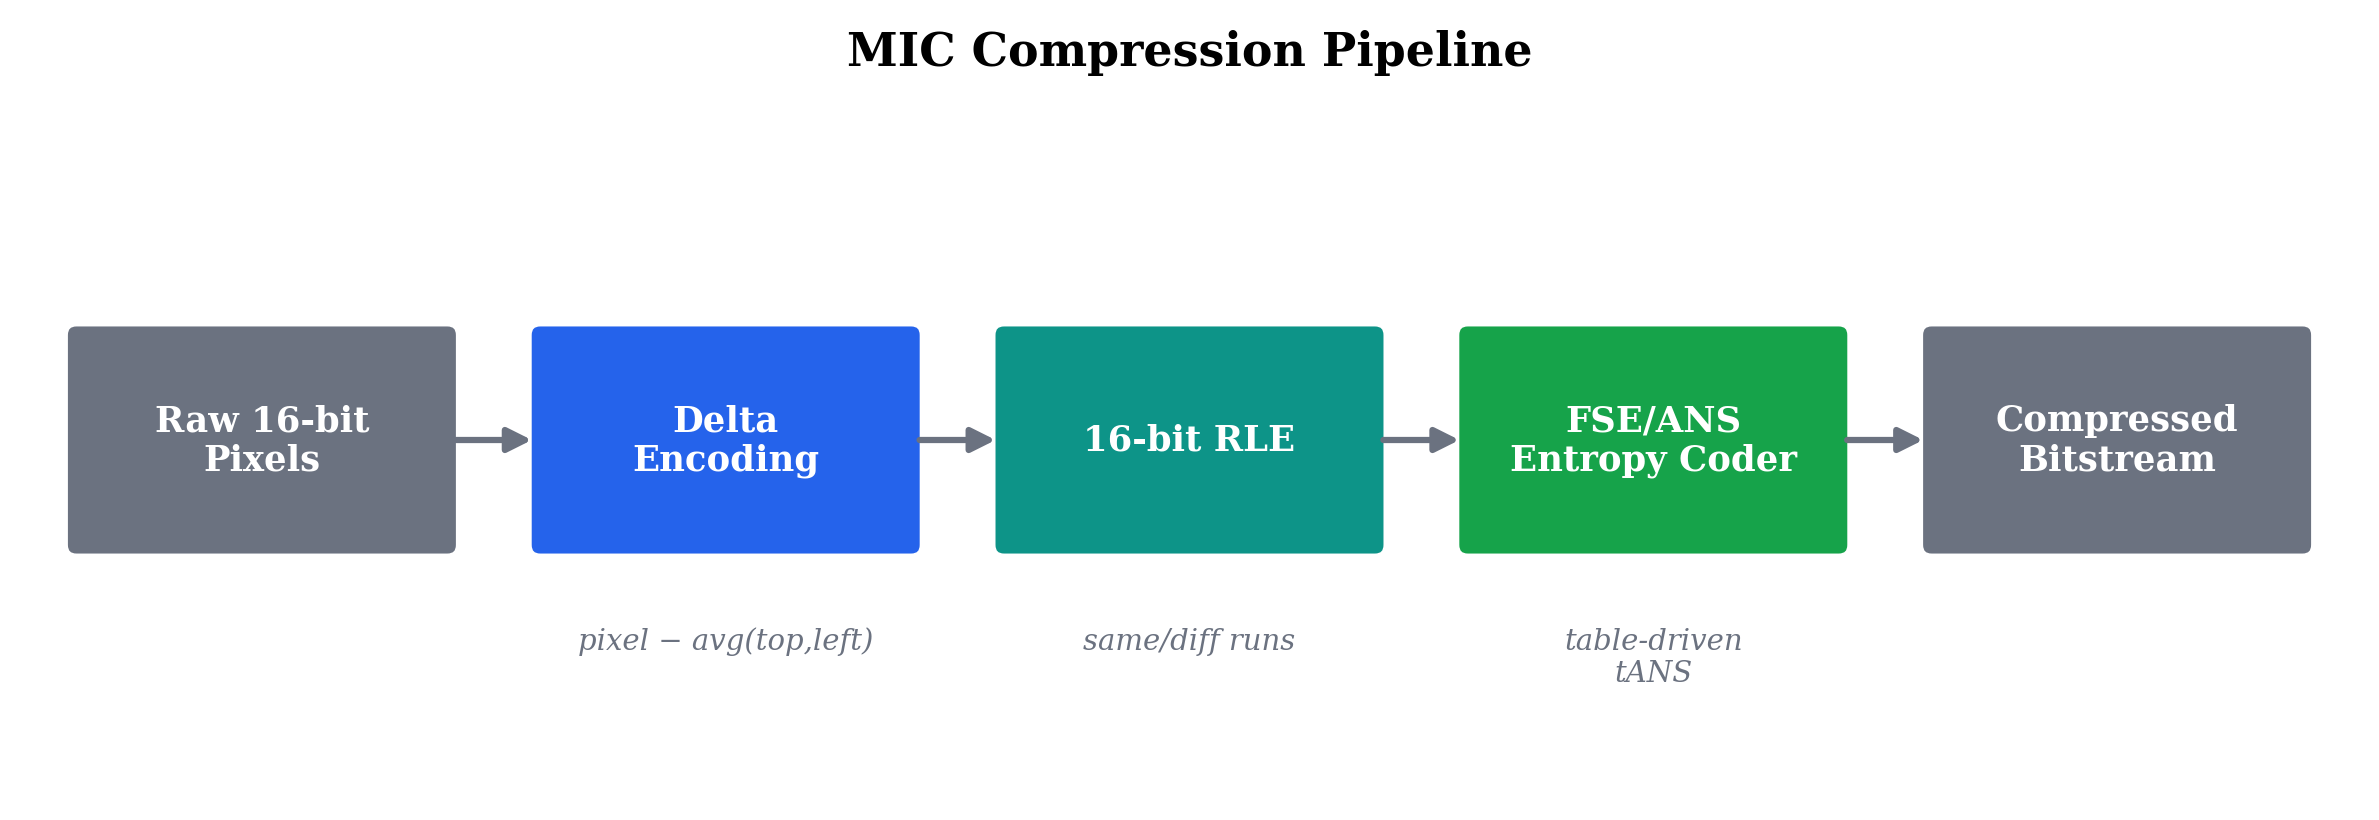
\includegraphics[width=0.85\textwidth]{figures/fig1_pipeline.png}
\caption{MIC compression pipeline. Raw 16-bit pixels are delta-encoded (avg of
top and left neighbors), run-length encoded (same/diff runs), and entropy-coded
with a 16-bit-native FSE/tANS coder.}
\label{fig:pipeline}
\end{figure*}

\subsection{Spatial Prediction}

Let $x_{i,j}$ denote the pixel at row $i$, column $j$. For interior pixels, MIC
predicts the current pixel from the average of the top and left neighbors:
\begin{equation}
  \hat{x}_{i,j} = \left\lfloor \frac{x_{i-1,j} + x_{i,j-1}}{2} \right\rfloor
\end{equation}
where the division is integer division rounded down (matching the decoder
exactly), and all arithmetic is performed in unsigned integers.
The residual is formed as:
\begin{equation}
  r_{i,j} = x_{i,j} - \hat{x}_{i,j}.
\end{equation}

Boundary pixels use only the available neighbor, and the first pixel is stored
directly. This predictor was selected because it is computationally simple,
branch-light in decoding, and effective on the current dataset.

\textbf{Predictor comparison.} We implemented and compared four predictors
through the full RLE\,+\,FSE pipeline on the 21-image dataset: left-only (left
neighbor, no top), average (MIC default), Paeth (PNG predictor~\cite{png}), and
MED (JPEG-LS~\cite{loco1}). Table~\ref{tab:predictor-summary} summarizes
geometric means and relative gains.

\begin{table}[htbp]
\centering
\caption{Predictor ablation summary: geometric means and win counts across all
21 images.}
\label{tab:predictor-summary}
\begin{tabular}{lrrr}
\toprule
Predictor & Geo.\ Mean & Wins & Avg$\to$X \\
\midrule
Left-only & 3.38$\times$ & 3/21 & $-$2.3\% \\
Average (MIC) & 3.46$\times$ & 13/21 & baseline \\
Paeth & 3.48$\times$ & 2/21 & $+$0.5\% \\
MED (JPEG-LS) & 3.52$\times$ & 16/21 & $+$1.6\% \\
\bottomrule
\end{tabular}
\end{table}

MED decompression is 1.5--2$\times$ slower due to the three-way conditional
branch and diagonal neighbor dependency that prevents the branch-free interior
loop used by the average predictor. MED yields the best geomean ratio
($+$1.6\% over Avg) but at significant speed cost; the average predictor is
retained as the default for its consistent per-modality performance and
branch-free decompression path.

\subsection{Effective Bit Depth and Overflow Coding}

For 16-bit images, residuals can span $[-65535, +65535]$. Rather than widening
the main residual stream to 32 bits, MIC uses an overflow delimiter scheme
derived from the effective image bit depth:
\begin{equation}
  d = \lceil \log_2(\max(x) + 1) \rceil.
\end{equation}

Residuals within an in-range interval are mapped directly to 16-bit codes.
Residuals outside that interval are encoded using a delimiter followed by the
raw pixel value.

\textbf{Encoding procedure:}
\begin{enumerate}
  \item Compute \texttt{deltaThreshold} $= 2^{d-1} - 1$.
  \item Compute delimiter $D = 2^d - 1$.
  \item For each residual $r_{i,j}$: if $|r_{i,j}| <$ \texttt{deltaThreshold},
  emit \texttt{uint16(deltaThreshold $+$ $r_{i,j}$)}; otherwise emit delimiter
  $D$, then emit raw pixel $x_{i,j}$.
\end{enumerate}

The threshold condition is strict ($<$, not $\leq$), so residuals with
$|r| =$ \texttt{deltaThreshold} take the overflow path. Residual zero maps
to code value \texttt{deltaThreshold} exactly. Table~\ref{tab:overflow-map}
illustrates the mapping for a representative bit depth.

\begin{table}[htbp]
\centering
\caption{Overflow coding example for $d=12$ bits
(\texttt{deltaThreshold}$=2047$, $D=4095$).}
\label{tab:overflow-map}
\scriptsize
\begin{tabular}{lll}
\toprule
Residual $r$ & Emitted code(s) & Notes \\
\midrule
$-2$ & $2045$ & in-range \\
$-1$ & $2046$ & in-range \\
$0$  & $2047$ & in-range (= threshold) \\
$+1$ & $2048$ & in-range \\
$+2$ & $2049$ & in-range \\
$\pm 2047$ & $4095$, raw pixel & overflow \\
\bottomrule
\end{tabular}
\end{table}

\textbf{Non-collision proof.} In-range residuals satisfy $|r| \leq$
\texttt{deltaThreshold}~$-$~$1$, so stored values range from 1 to $2^d - 3$.
The delimiter is $D = 2^d - 1$. Since $2^d - 3 < 2^d - 1$, the stored value of
a direct residual can never equal $D$; the two ranges are disjoint.

\textbf{Decoding procedure:} Read the next uint16 value $c$.
If $c \neq D$, recover the residual as $r = \texttt{int16}(c -$
\texttt{deltaThreshold}$)$ and reconstruct $x_{i,j} = \hat{x}_{i,j} + r$.
If $c = D$, the raw pixel follows: read the next uint16 as $x_{i,j}$ directly.

\subsection{16-Bit Run-Length Encoding}

The predicted residual stream is converted into an alternating sequence of:
\begin{itemize}
  \item \textbf{Same runs}: a count and a repeated 16-bit value;
  \item \textbf{Diff runs}: a count followed by a sequence of distinct 16-bit
  values.
\end{itemize}

A same run is emitted only when at least three consecutive identical values are
observed.

\textbf{Midpoint protocol.} Run headers are stored as uint16 values. A
midpoint constant \texttt{midCount}$= 32767$ partitions the header space: a
count $c \leq$ \texttt{midCount} signals a same run of length $c$; a count
$c >$ \texttt{midCount} signals a diff run of length $c -$ \texttt{midCount}.
The maximum same-run or diff-run length is therefore 32767 symbols; longer
sequences are split into multiple headers transparently. The decoder
distinguishes the two run types solely by comparing the header value against
\texttt{midCount}.

\textbf{Encoding example.} For the residual code sequence
$[5,5,5,5,9,10,11,11,11]$, the RLE output is:
same($c=4$, value=$5$), diff($c=2$, values=$9,10$), same($c=3$, value=$11$).
The encoded stream contains five uint16 words: $[4,\ 5,\ 32769,\ 9,\ 10,\ 3,\ 11]$,
where $32769 = \texttt{midCount} + 2$ signals a diff run of length 2.

\textbf{Why 16-bit RLE matters.} A run of 1,000 identical 16-bit residuals
$v = \texttt{0x0103}$ is encoded by MIC as two uint16 words (a count and the
value), regardless of $v$'s byte pattern. A byte-oriented RLE sees the
interleaved stream $\texttt{0x03,0x01,0x03,0x01,\ldots}$: no single byte
repeats 1,000 times, so it must emit two interleaved runs or fall back to
literals.

\textbf{Same-run fast path.} Same-value runs (often $>$80\% of all runs on
smooth medical images after delta coding) are fast-pathed in the decoder to
return the cached value without touching the compressed-data slice. Each output
symbol in a same run requires only a counter decrement.

\subsection{Large-Alphabet FSE Coding}

\textbf{FSE overview.} FSE maintains a single integer \emph{state}. To decode
one symbol, the decoder indexes a prebuilt decode table using the current state.
Each table entry stores the output symbol, the number of bits $n$ to read from
the bitstream, and a base value $b$ for the next state. The decoder reads $n$
bits from the bitstream and computes the next state as $b +$ (bits read). This
requires only a table lookup, a bit read, and an addition per symbol; no
divisions or multiplications are needed. \textbf{Encoding} processes symbols in
reverse order (last symbol first), building the compressed bitstream from the
end; \textbf{decoding} reads bits forward.

The RLE output is entropy-coded using table-based ANS (tANS), implemented as
Finite State Entropy. MIC extends FSE to support up to 65,535 distinct symbols.
As noted in Section~\ref{sec:intro}, one 16-bit code value is reserved as the
overflow delimiter, leaving at most 65,535 codes available for residual symbols.
This contrasts with the 4,096-symbol limit in Zstandard's FSE implementation,
which was designed for byte-oriented streams.

\textbf{Dynamic table sizing.} Encode and decode tables are sized to the actual
observed symbol range rather than the theoretical maximum. For 8-bit
images stored in 16-bit containers (common in MR), this reduces the working set
from 512\,KB to approximately 2\,KB.

\subsection{Adaptive Table Size Selection}

The FSE \emph{tableLog} parameter determines the size of the decode table
($2^{\textit{tableLog}}$ entries) and the precision of symbol probability
estimates. MIC automatically selects tableLog based on the number of active
symbols and observation density:
\begin{itemize}
  \item $\textit{symbolLen}$ = number of distinct symbols observed in the RLE
  output stream (equivalently, the observed symbol range: max value minus
  min value plus 1, counting all positions in that range even if some go
  unused).
  \item $\textit{inputLength}$ = total number of symbols in the RLE output
  stream fed to the FSE coder.
  \item $\textit{symbolDensity} = \textit{inputLength} / \textit{symbolLen}$,
  i.e., average observations per symbol slot.
\end{itemize}

Selection rules:
\begin{itemize}
  \item Default $\textit{tableLog} = 11$.
  \item Bumped to 12 when $\textit{symbolDensity} > 32$ and
  $\textit{symbolLen} > 128$.
  \item Bumped to 13 when $\textit{symbolLen} > 512$ and
  $\textit{symbolDensity} > 16$.
\end{itemize}

Table~\ref{tab:tablelog-ablation} presents the tableLog ablation across
selected images.

\begin{table}[htbp]
\centering
\caption{TableLog ablation: forced TL=11/12/13 vs.\ adaptive selection
(selected images, Apple M2 Max).}
\label{tab:tablelog-ablation}
\scriptsize
\begin{tabular}{lrrrr}
\toprule
Image & TL=11 & TL=12 & TL=13 & Adaptive \\
\midrule
CR  & 3.47$\times$ & 3.63$\times$ & 3.69$\times$ & 3.69$\times$ \\
MG1 & 8.00$\times$ & 8.57$\times$ & 8.79$\times$ & 8.79$\times$ \\
MG2 & 7.98$\times$ & 8.55$\times$ & 8.77$\times$ & 8.77$\times$ \\
MR2 & 3.14$\times$ & 3.24$\times$ & 3.28$\times$ & 3.28$\times$ \\
RG2 & 3.85$\times$ & 4.12$\times$ & 4.23$\times$ & 4.23$\times$ \\
RG3 & 5.64$\times$ & 5.95$\times$ & 6.08$\times$ & 6.08$\times$ \\
\bottomrule
\end{tabular}
\end{table}

Nine images benefit from TL=12 or TL=13 (CR $+$6.3\%, MG1 $+$9.9\%, MG2
$+$9.9\%, MR2 $+$4.6\%, RG2 $+$9.9\%, RG3 $+$7.8\%, XA1 $+$4.4\%, MR3
$+$0.9\%, NM1 $+$1.9\%); the adaptive policy correctly identifies all
beneficial cases. Decompression throughput is unaffected by tableLog choice
($<$5\% variation).


% ============================================================
\section{Multi-State Entropy Decoding}
\label{sec:multistate}

\subsection{The Serial Dependency Problem}

A conventional single-state table-based ANS decoder contains a serial
dependency chain:
\begin{equation}
\begin{aligned}
  \text{let } e &= \texttt{decTable}[s_n], \\
  s_{n+1} &= e.\textit{newState} + \texttt{getBits}(e.\textit{nbBits}).
\end{aligned}
\end{equation}
With a table-lookup latency of approximately $L \approx 4$ cycles on modern
out-of-order CPUs (L1 cache hit), the loop is limited to roughly one symbol per
$L$ cycles regardless of available execution units. Modern CPUs have 4--6
execution ports; a single-state ANS decoder uses exactly one dependency chain,
leaving 75--83\% of the hardware capacity idle.

\subsection{Interleaved Decoding}

MIC breaks this dependency by running multiple independent state machines on
interleaved symbol positions. In the four-state design, four independent chains
(A, B, C, D) reconstruct positions:
\begin{align*}
  \text{chain A}&: 0, 4, 8, \ldots \\
  \text{chain B}&: 1, 5, 9, \ldots \\
  \text{chain C}&: 2, 6, 10, \ldots \\
  \text{chain D}&: 3, 7, 11, \ldots
\end{align*}

The four chains are completely independent: each has its own state variable, its
own sequence of table lookups, and its own bit-extraction operations. The CPU's
out-of-order engine sees four simultaneous table-lookup address streams.

\textbf{Bitstream format.} The encoder partitions the output symbol sequence
into four interleaved subsequences, encodes each independently (producing four
FSE-compressed streams), and concatenates them. The four stream lengths are
stored as a 4-entry header so the decoder can locate each stream's start
offset. All four chains use the same FSE decode table (built from the joint
histogram over all symbols). Initial state values for each chain are stored as
part of the per-chain header. Output reordering is performed by the decoder,
which writes reconstructed symbols to positions $4k$, $4k+1$, $4k+2$, $4k+3$
from chains A, B, C, D respectively.

\textbf{Latency model.} Let $L$ be the table-lookup latency (cycles).
Single-state FSE processes 1 symbol per $L$ cycles. The $k$-state decoder
processes $k$ symbols per $L$ cycles (amortized):

\begin{table}[htbp]
\centering
\caption{Multi-state decoder latency model and empirical speedup.}
\label{tab:latency}
\begin{tabular}{clrr}
\toprule
States ($k$) & Amortized latency & Theoretical & Empirical \\
\midrule
1 & $L$ cy/sym & 1.0$\times$ & 1.0$\times$ \\
2 & $L/2$ cy/sym & 2.0$\times$ & 1.3$\times$ \\
4 & $L/4$ cy/sym & 4.0$\times$ & 2.0$\times$ \\
\bottomrule
\end{tabular}
\end{table}

The empirical speedup is below theoretical maximum due to: (1) bit-reader
refill overhead shared across all chains, (2) instruction cache pressure from
the unrolled loop, and (3) memory bandwidth limits on compressed stream
reads~\cite{williams2009}.

\subsection{Correctness and Signaling}
\label{sec:signaling}

Correctness follows from partitioning the output sequence into independent
subsequences during encoding and reversing that assignment during decoding;
each chain operates on a strict subset of positions with no cross-chain data
dependency.

The bitstream signals the decoding mode with a 2-byte magic header:
\texttt{0xFF,0x02} for two-state; \texttt{0xFF,0x04} for four-state; followed
by a 4-byte symbol count. In the single-state format, the first byte encodes
\texttt{tableLog}. Since the maximum supported \texttt{tableLog} is 17, a first
byte of \texttt{0xFF} ($= 255$) is not a valid single-state \texttt{tableLog}
value and can safely be reused as the extended-format marker. All three formats
coexist without ambiguity.

\textbf{Platform-specific kernels.} On AMD64, Bit Manipulation Instruction
Set 2 (BMI2) \texttt{SHLXQ}/\texttt{SHRXQ} instructions provide 3-operand
variable shifts without contention on the \texttt{CL} register (the x86 shift
count register used by traditional variable shifts); on ARM64,
\texttt{LSLV}/\texttt{LSRV} (logical shift left/right variable) serve the same
role natively. Pure-Go implementations cover all other targets.

\subsection{Isolated FSE Decompression Throughput}

Table~\ref{tab:fse-combined} reports isolated FSE decompression throughput
(MB/s over the uncompressed RLE symbol stream) for a representative subset of
modalities on both platforms.

\begin{table}[htbp]
\centering
\caption{Isolated FSE decompression throughput (MB/s) for representative
modalities. ARM64: Apple M2 Max, pure Go. AMD64: Intel Core Ultra 9 285K,
4-state uses BMI2 assembly (\texttt{fse4StateDecompKernel}).}
\label{tab:fse-combined}
\scriptsize
\begin{tabular}{lrrrrrr}
\toprule
 & \multicolumn{3}{c}{ARM64 (MB/s)} & \multicolumn{3}{c}{AMD64 (MB/s)} \\
\cmidrule(lr){2-4}\cmidrule(lr){5-7}
Image & 1-st & 4-st & gain & 1-st & 4-st & gain \\
\midrule
MR   &   514 &   841 & $+$64\% &   600 &   828 & $+$38\% \\
CT   &   829 & 1,295 & $+$56\% &   941 & 1,631 & $+$73\% \\
CR   &   140 &   966 & $+$590\%$^*$ & 1,994 & 4,535 & $+$127\% \\
XR   & 1,444 & 1,952 & $+$35\% & 3,195 & 5,771 & $+$81\% \\
MG1  & 1,140 & 1,873 & $+$64\% & 3,379 & 4,952 & $+$47\% \\
MG-N & 2,944 & 5,696 & $+$94\% & 2,722 & 4,981 & $+$83\% \\
NM1  & 1,658 & 2,254 & $+$36\% & 2,078 & 2,407 & $+$16\% \\
RG1  & 1,676 & 3,128 & $+$87\% & 2,506 & 4,336 & $+$73\% \\
\midrule
\textbf{Geomean (21)} & \textbf{1,418} & \textbf{2,375} & \textbf{$+$68\%} &
\textbf{2,309} & \textbf{3,306} & \textbf{$+$43\%} \\
\bottomrule
\end{tabular}
\end{table}

$^*$CR single-state is depressed by the \texttt{zeroBits} bounds-check path
(triggered when any symbol probability exceeds 50\%); multi-state interleaving
reduces this overhead. The AMD64 BMI2 kernel sidesteps the pure-Go check
entirely, yielding $+$127\%.

The 4-state decoder delivers a geometric-mean speedup of $+$68\% on ARM64 and
$+$43\% on AMD64 over the 1-state baseline. The smaller AMD64 gain reflects
a higher 1-state baseline: the Intel out-of-order engine tolerates the serial
dependency chain more efficiently, compressing the relative multi-state
improvement. For C and SIMD variant throughput on AMD64, see
Table~\ref{tab:decomp-amd64}.

% ============================================================
\section{Experimental Methodology}
\label{sec:methodology}

\subsection{Dataset}

The evaluation uses 21 de-identified DICOM images spanning 10 modalities, drawn
from publicly available datasets: NEMA WG-04 compsamples, NEMA 1997 CD, and the
Clunie Breast Tomosynthesis Case~1 (Table~\ref{tab:dataset}). All images are
de-identified per DICOM PS 3.15 Appendix~E; no ethics approval is required.

\begin{table}[htbp]
\centering
\caption{Test dataset: 21 clinical DICOM images spanning 10 modalities.}
\label{tab:dataset}
\scriptsize
\begin{tabular}{llrr}
\toprule
Image & Modality & Dimensions & Raw (MB) \\
\midrule
MR   & Brain MRI      & $256{\times}256$   & 0.13 \\
CT   & CT scan        & $512{\times}512$   & 0.50 \\
CR   & Comp.\ radiography & $2140{\times}1760$ & 7.18 \\
XR   & X-ray          & $2048{\times}2577$ & 10.1 \\
MG1  & Mammography    & $2457{\times}1996$ & 9.35 \\
MG2  & Mammography    & $2457{\times}1996$ & 9.35 \\
MG3  & Mammography    & $4774{\times}3064$ & 27.3 \\
MG4  & Mammography    & $4096{\times}3328$ & 26.0 \\
CT1  & CT scan        & $512{\times}512$   & 0.50 \\
CT2  & CT scan        & $512{\times}512$   & 0.50 \\
MG-N & Mammography    & $3064{\times}4664$ & 27.3 \\
MR1  & Brain MRI      & $512{\times}512$   & 0.50 \\
MR2  & Brain MRI      & $1024{\times}1024$ & 2.00 \\
MR3  & Brain MRI      & $512{\times}512$   & 0.50 \\
MR4  & Brain MRI      & $512{\times}512$   & 0.50 \\
NM1  & Nuclear med.   & $256{\times}1024$  & 0.50 \\
RG1  & Radiography    & $1841{\times}1955$ & 6.86 \\
RG2  & Radiography    & $1760{\times}2140$ & 7.18 \\
RG3  & Radiography    & $1760{\times}1760$ & 5.91 \\
SC1  & Sec.~capture   & $2048{\times}2487$ & 9.71 \\
XA1  & Fluoroscopy    & $1024{\times}1024$ & 2.00 \\
\bottomrule
\end{tabular}
\end{table}

This dataset spans multiple modalities and image sizes but remains modest for
strong generalization claims.

\subsection{Baselines}

The current study compares MIC with:
\begin{itemize}
  \item \textbf{HTJ2K} (OpenJPH~\cite{openjph}), via in-process CGO bindings,
  \item \textbf{JPEG-LS} (CharLS~\cite{charls}), via in-process CGO bindings,
  and
  \item \textbf{Delta\,+\,Zstandard} (level 19).
\end{itemize}

\subsection{Metrics}

The paper reports:
\begin{itemize}
  \item \textbf{Compression ratio}: uncompressed size / compressed size.
  \item \textbf{Decompression throughput}: uncompressed pixel bytes
  reconstructed per second (MB/s).
  \item \textbf{Encoding throughput}: uncompressed pixel bytes processed per
  second (MB/s).
\end{itemize}

\subsection{Benchmark Procedure}

All codecs were measured using in-process library calls on the same machine to
avoid file-I/O and subprocess overhead. The Go testing framework's
\texttt{-benchtime=10x} flag was used (10 iterations per benchmark; each
iteration processes the full image). Run-to-run variance is $<$2\% on Apple
M2 Max and $<$5\% on Intel AMD64.

\textbf{Platforms and compiler flags:}
\begin{itemize}
  \item Apple M2 Max (12-core ARM64), macOS. Go compiler (gc) with default
  optimization; CGO-linked C components compiled with \texttt{-O3}.
  \item Intel Core Ultra 9 285K (x86-64/AMD64, mixed P-core/E-core topology),
  Linux. Go compiler (gc) with default optimization; C components compiled
  with \texttt{-O3 -march=native}.
\end{itemize}

\textbf{Codec variants}:
\begin{itemize}
  \item \textbf{MIC-Go}: Pure Go, single-state FSE decoder.
  \item \textbf{MIC-4state}: Pure Go, four-state FSE decoder.
  \item \textbf{MIC-4state-C}: C four-state FSE decoder via CGO.
  \item \textbf{MIC-4state-SIMD}: C four-state FSE with BMI2 (AMD64) or scalar
  (ARM64) via CGO.
  \item \textbf{Wavelet+SIMD}: 5/3 wavelet with blocked column layout and
  Advanced Vector Extensions 2 (AVX2) kernels (AMD64) or scalar blocked
  (ARM64).
  \item \textbf{PICS-C-$N$}: Parallel Image Compressed Strips, a strip-parallel
  mode that splits the image into $N$ horizontal strips, compresses each
  strip independently with its own FSE table, and decompresses all strips
  in parallel using a C pthreads worker pool. Strips are independently
  decodable.
\end{itemize}


\subsection{JavaScript and Browser Evaluation}

A pure JavaScript decoder (${\sim}$20\,KB ES module, zero Node Package Manager
(npm) dependencies) and a Go WebAssembly build (${\sim}$2.5\,MB) were
implemented. Performance measurements reported in Section~\ref{sec:results}
were obtained in Node.js v24.8 (Apple M2 Max).

% ============================================================
\section{Results}
\label{sec:results}

\subsection{Compression Ratio}

Table~\ref{tab:ratios} presents lossless compression ratios for all codec
variants across the 21-image dataset.

\begin{table*}[t]
\centering
\caption{Lossless compression ratios: all codec variants, 21 images. Bold =
best ratio per row.}
\label{tab:ratios}
\scriptsize
\begin{tabular}{lrrrrrrrr}
\toprule
Image & Raw (MB) & $\Delta$+Zstd-19 & MIC & Wavelet & PICS-4 & PICS-8 & HTJ2K & JPEG-LS \\
\midrule
MR   & 0.13 & 1.95$\times$ & 2.35$\times$ & 2.38$\times$ & 2.28$\times$ & 2.21$\times$ & 2.38$\times$ & \textbf{2.52$\times$} \\
CT   & 0.50 & 2.05$\times$ & 2.24$\times$ & 1.67$\times$ & 2.15$\times$ & 1.96$\times$ & 1.77$\times$ & \textbf{2.68$\times$} \\
CR   & 7.18 & 3.24$\times$ & 3.69$\times$ & 3.81$\times$ & 3.70$\times$ & 3.71$\times$ & 3.77$\times$ & \textbf{3.96$\times$} \\
XR   & 10.1 & 1.43$\times$ & 1.74$\times$ & \textbf{1.76$\times$} & 1.75$\times$ & \textbf{1.76$\times$} & 1.67$\times$ & \textbf{1.76$\times$} \\
MG1  & 9.35 & 7.20$\times$ & 8.79$\times$ & 8.67$\times$ & 8.84$\times$ & 8.87$\times$ & 8.25$\times$ & \textbf{8.91$\times$} \\
MG2  & 9.35 & 7.21$\times$ & 8.77$\times$ & 8.65$\times$ & 8.83$\times$ & 8.85$\times$ & 8.24$\times$ & \textbf{8.90$\times$} \\
MG3  & 27.3 & 2.04$\times$ & 2.24$\times$ & 2.32$\times$ & 2.31$\times$ & 2.34$\times$ & 2.22$\times$ & \textbf{2.38$\times$} \\
MG4  & 26.0 & 3.10$\times$ & 3.47$\times$ & 3.59$\times$ & 3.59$\times$ & 3.62$\times$ & 3.51$\times$ & \textbf{3.71$\times$} \\
CT1  & 0.50 & 2.47$\times$ & 2.79$\times$ & 2.49$\times$ & 2.54$\times$ & 2.29$\times$ & 2.70$\times$ & \textbf{3.19$\times$} \\
CT2  & 0.50 & 3.24$\times$ & 3.49$\times$ & 2.87$\times$ & 3.11$\times$ & 2.72$\times$ & 3.29$\times$ & \textbf{4.54$\times$} \\
MG-N & 27.3 & 2.04$\times$ & 2.24$\times$ & 2.32$\times$ & 2.31$\times$ & 2.34$\times$ & 2.23$\times$ & \textbf{2.38$\times$} \\
MR1  & 0.50 & 1.79$\times$ & 2.09$\times$ & 2.14$\times$ & 2.10$\times$ & 2.08$\times$ & 2.13$\times$ & \textbf{2.30$\times$} \\
MR2  & 2.00 & 2.77$\times$ & 3.28$\times$ & 3.34$\times$ & 3.31$\times$ & 3.31$\times$ & 3.35$\times$ & \textbf{3.52$\times$} \\
MR3  & 0.50 & 3.47$\times$ & 3.93$\times$ & 4.09$\times$ & 3.89$\times$ & 3.84$\times$ & 4.33$\times$ & \textbf{4.51$\times$} \\
MR4  & 0.50 & 3.58$\times$ & 4.12$\times$ & 4.18$\times$ & 4.09$\times$ & 4.03$\times$ & 4.21$\times$ & \textbf{4.49$\times$} \\
NM1  & 0.50 & 4.88$\times$ & 5.15$\times$ & 5.02$\times$ & 5.26$\times$ & 5.28$\times$ & 5.76$\times$ & \textbf{6.28$\times$} \\
RG1  & 6.86 & 1.45$\times$ & 1.70$\times$ & 1.70$\times$ & 1.70$\times$ & 1.69$\times$ & 1.63$\times$ & \textbf{1.72$\times$} \\
RG2  & 7.18 & 3.68$\times$ & 4.23$\times$ & 4.32$\times$ & 4.28$\times$ & 4.30$\times$ & 4.32$\times$ & \textbf{4.51$\times$} \\
RG3  & 5.91 & 5.46$\times$ & 6.08$\times$ & 6.82$\times$ & 6.11$\times$ & 6.12$\times$ & 6.99$\times$ & \textbf{7.31$\times$} \\
SC1  & 9.71 & 3.46$\times$ & 3.71$\times$ & 3.70$\times$ & 3.73$\times$ & 3.74$\times$ & 3.85$\times$ & \textbf{4.73$\times$} \\
XA1  & 2.00 & 4.37$\times$ & 5.01$\times$ & 4.94$\times$ & 5.04$\times$ & 5.03$\times$ & 4.88$\times$ & \textbf{5.39$\times$} \\
\bottomrule
\end{tabular}
\end{table*}


\textbf{Analysis.} JPEG-LS achieves the highest lossless ratio on all 21
images, as expected given its context-adaptive MED predictor. MIC's design
target is not ratio alone but the ratio-throughput-simplicity tradeoff: on
ARM64, MIC-4state-C achieves approximately 91\% of JPEG-LS's geometric mean
ratio (3.12$\times$ vs.\ 3.44$\times$) while delivering approximately
4$\times$ the single-threaded decompression throughput and requiring about
1/5 the source lines.

Mammography achieves the highest MIC ratios (up to 8.79$\times$) due to smooth
tissue regions producing near-zero RLE runs. CT with full 16-bit dynamic range
achieves 2.24$\times$ (MIC) vs.\ 1.67$\times$ (Wavelet): coefficient overflow
in the 5/3 lifting step inflates Wavelet compressed size.

\textbf{PICS strip adaptation.} Each PICS strip receives a dedicated FSE table
that specializes to its local residual distribution. On large images, this
per-strip specialization improves ratio slightly because
$\sum_k |S_k| \cdot H(S_k) < |S| \cdot H(S)$ when residual statistics vary
across strips.

\subsection{Effect of 16-Bit-Native Residual Coding}

MIC outperforms Delta+Zstandard (zstd level 19) by 5--22\% on all 21 tested
images (geometric mean $+$14\%). The gap is structural: the mutual information
$I(X_H;\, X_L)$ of delta residuals ranges from 0.3\,bits/symbol (MR) to
1.1\,bits/symbol (MG3), matching the empirical range.

\subsection{Decompression Throughput---ARM64}

Table~\ref{tab:decomp-arm} presents decompression throughput on Apple M2 Max.
MIC-4state-C is the fastest single-threaded decoder on 13/21 images; PICS-C-8
exceeds HTJ2K on all 21 images.

\begin{table*}[t]
\centering
\caption{Decompression throughput (MB/s), Apple M2 Max (ARM64). Bold = fastest
per row (single-threaded: first 5 cols; PICS: last 3 cols).}
\label{tab:decomp-arm}
\scriptsize
\begin{tabular}{lrrrrrrrr}
\toprule
Image & MIC-Go & MIC-4s-C & Wav+SIMD & HTJ2K & JPEG-LS & PICS-C-2 & PICS-C-4 & PICS-C-8 \\
\midrule
MR   & 144 & \textbf{348} & 248 & 265 & 102 & 530 & \textbf{710}$^\dagger$ & 482 \\
CT   & 191 & \textbf{356} & 316 & 307 & 137 & 524 & 955 & \textbf{1,092} \\
CR   & 296 & 524 & \textbf{567} & 367 & 153 & 867 & 1,635 & \textbf{2,661} \\
XR   & 308 & 533 & \textbf{627} & 334 & 108 & 874 & 1,666 & \textbf{3,025} \\
MG1  & 482 & 683 & 678 & \textbf{810} & 409 & 1,205 & 2,112 & \textbf{3,656} \\
MG2  & 479 & 686 & 697 & \textbf{790} & 416 & 1,225 & 2,120 & \textbf{3,773} \\
MG3  & 308 & \textbf{531} & 422 & 338 & 153 & 864 & 1,673 & \textbf{3,117} \\
MG4  & 417 & \textbf{625} & 516 & 548 & 184 & 1,093 & 2,004 & \textbf{3,689} \\
CT1  & 239 & \textbf{436} & 425 & 362 & 182 & 686 & 1,013 & \textbf{1,183} \\
CT2  & 238 & 439 & \textbf{481} & 375 & 175 & 676 & 1,041 & \textbf{1,189} \\
MG-N & 316 & \textbf{536} & 468 & 340 & 153 & 883 & 1,711 & \textbf{3,175} \\
MR1  & 278 & \textbf{521} & 435 & 325 & 116 & 751 & 1,207 & \textbf{1,402} \\
MR2  & 333 & \textbf{563} & 498 & 388 & 172 & 913 & 1,552 & \textbf{2,466} \\
MR3  & 375 & \textbf{639} & 507 & 441 & 236 & 908 & 1,430 & \textbf{1,614} \\
MR4  & 316 & \textbf{571} & 479 & 406 & 197 & 818 & 1,341 & \textbf{1,558} \\
NM1  & 327 & \textbf{632} & 575 & 410 & 210 & 888 & 1,400 & \textbf{1,679} \\
RG1  & 235 & 406 & \textbf{584} & 332 & 104 & 602 & 1,128 & \textbf{2,017} \\
RG2  & 367 & 590 & \textbf{644} & 443 & 193 & 986 & 1,803 & \textbf{3,194} \\
RG3  & 374 & 604 & \textbf{656} & 562 & 246 & 1,035 & 1,944 & \textbf{3,302} \\
SC1  & 375 & \textbf{587} & 388 & 401 & 229 & 1,017 & 1,861 & \textbf{3,279} \\
XA1  & 331 & \textbf{576} & 459 & 419 & 204 & 928 & 1,583 & \textbf{2,493} \\
\bottomrule
\end{tabular}
\end{table*}

$^\dagger$MR is too small for PICS-C-8; PICS-C-4 is best.
MIC-4state-C is 1.7--5.0$\times$ faster than JPEG-LS on all 21 images.
PICS-C-8 peaks at 3,773\,MB/s on MG2.

\subsection{Decompression Throughput---AMD64}

Table~\ref{tab:decomp-amd64} presents results on AMD64 where MIC-4state-SIMD
activates BMI2/PDEP and Wavelet+SIMD gains AVX2 kernels.

\begin{table*}[t]
\centering
\caption{Decompression throughput (MB/s), Intel Core Ultra 9 285K (AMD64).
Bold = fastest per row within single-threaded and PICS groups.}
\label{tab:decomp-amd64}
\scriptsize
\begin{tabular}{lrrrrrrr}
\toprule
Image & MIC-Go & MIC-4s-C & MIC-4s-SIMD & Wav+SIMD & HTJ2K & PICS-C-4 & PICS-C-8 \\
\midrule
MR   & 251 & 501 & \textbf{708} & 194 & 570 & 301 & 124$^\dagger$ \\
CT   & 231 & 403 & 487 & 364 & \textbf{544} & \textbf{676} & 339 \\
CR   & 324 & 599 & \textbf{744} & 723 & 708 & 1,738 & \textbf{2,435} \\
XR   & 363 & 601 & \textbf{803} & 681 & 570 & 1,714 & \textbf{1,994} \\
MG1  & 617 & 789 & 1,119 & 746 & \textbf{1,235} & 1,872 & \textbf{2,514} \\
MG2  & 562 & 800 & 1,166 & 848 & \textbf{1,297} & \textbf{2,244} & 2,085 \\
MG3  & 357 & 633 & 669 & \textbf{678} & 644 & 1,823 & \textbf{2,538} \\
MG4  & 523 & 743 & 773 & \textbf{808} & 916 & 2,124 & \textbf{2,707} \\
CT1  & 322 & 520 & \textbf{676} & 525 & 657 & \textbf{857} & 423 \\
CT2  & 293 & 514 & 636 & \textbf{705} & 627 & \textbf{847} & 687 \\
MG-N & 368 & 635 & 669 & \textbf{705} & 643 & 1,872 & \textbf{2,191} \\
MR1  & 356 & 609 & \textbf{766} & 532 & 654 & \textbf{945} & 366 \\
MR2  & 352 & 658 & \textbf{975} & 601 & 749 & \textbf{1,121} & 793 \\
MR3  & 450 & 728 & \textbf{809} & 676 & 802 & \textbf{920} & 705 \\
MR4  & 390 & 596 & \textbf{861} & 738 & 660 & 493 & \textbf{701} \\
NM1  & 367 & \textbf{717} & 668 & 715 & 627 & \textbf{783} & 405 \\
RG1  & 302 & 497 & 593 & \textbf{705} & 557 & 1,248 & \textbf{1,494} \\
RG2  & 433 & 676 & \textbf{861} & 811 & 823 & 1,841 & \textbf{1,912} \\
RG3  & 460 & 706 & 858 & 881 & \textbf{894} & \textbf{1,969} & 1,613 \\
SC1  & 464 & 695 & \textbf{888} & 710 & 728 & 1,819 & \textbf{1,889} \\
XA1  & 413 & 693 & \textbf{836} & 538 & 797 & 1,173 & \textbf{1,513} \\
\bottomrule
\end{tabular}
\end{table*}

$^\dagger$\textbf{MR} is too small for PICS-C-8; PICS-C-4 achieves the highest
PICS throughput on this image.

On AMD64, MIC-4state-SIMD leads 16/21 images single-threaded; HTJ2K leads on
MG1, MG2, MG4, CT, and RG3. PICS-C-8 exceeds HTJ2K on all 21 images on both
platforms.

\subsection{Encoding Throughput}

Tables~\ref{tab:enc-amd64} and~\ref{tab:enc-arm64-full} report per-image
encoding throughput for all codec variants on AMD64 and ARM64 respectively.
On ARM64, MIC-4state-C is 2--2.5$\times$ faster to encode than pure-Go
MIC-Go; JPEG-LS is consistently 2--4$\times$ slower than MIC-Go. PICS-8
reaches 1.2--2.1\,GB/s on large images, sufficient for real-time PACS
ingestion.

\begin{table*}[htbp]
\centering
\caption{Encoding throughput (MB/s), Intel Core Ultra 9 285K (AMD64). Bold =
fastest per row.}
\label{tab:enc-amd64}
\scriptsize
\begin{tabular}{lrrrrrrrr}
\toprule
Image & MIC-Go & MIC-4s-C & MIC-C & Wav+SIMD & HTJ2K & JPEG-LS & PICS-4 & PICS-8 \\
\midrule
MR  & 121 & \textbf{290} & 273 & 85 & 177 & 71 & 186 & 128 \\
CT  & 180 & \textbf{359} & 311 & 84 & 178 & 104 & 301 & 312 \\
CR  & 233 & 461 & 423 & 120 & 193 & 89 & 732 & \textbf{1,102} \\
XR  & 254 & 550 & 519 & 127 & 214 & 95 & 775 & \textbf{1,212} \\
MG1 & 380 & 861 & 820 & 155 & 508 & 239 & 1,112 & \textbf{1,651} \\
MG2 & 380 & 857 & 830 & 153 & 507 & 235 & 1,119 & \textbf{1,676} \\
MG3 & 256 & 556 & 514 & 97 & 202 & 109 & 832 & \textbf{1,317} \\
MG4 & 336 & 738 & 710 & 107 & 354 & 162 & 1,098 & \textbf{1,901} \\
CT1 & 206 & \textbf{413} & 384 & 94 & 216 & 132 & 310 & 329 \\
CT2 & 192 & \textbf{371} & 340 & 89 & 194 & 132 & 320 & 294 \\
MG-N & 254 & 562 & 529 & 99 & 202 & 107 & 842 & \textbf{1,353} \\
MR1 & 221 & \textbf{460} & 429 & 101 & 195 & 92 & 364 & 347 \\
MR2 & 275 & 566 & 532 & 107 & 230 & 102 & 643 & \textbf{857} \\
MR3 & 300 & \textbf{609} & 591 & 119 & 292 & 142 & 498 & 448 \\
MR4 & 249 & \textbf{494} & 451 & 108 & 226 & 142 & 370 & 368 \\
NM1 & 237 & \textbf{467} & 444 & 117 & 242 & 132 & 360 & 302 \\
RG1 & 229 & 485 & 397 & 123 & 198 & 70 & 651 & \textbf{942} \\
RG2 & 280 & 582 & 488 & 125 & 254 & 112 & 842 & \textbf{1,220} \\
RG3 & 275 & 550 & 512 & 128 & 273 & 143 & 863 & \textbf{1,222} \\
SC1 & 286 & 577 & 551 & 83 & 235 & 169 & 924 & \textbf{1,425} \\
XA1 & 242 & 496 & 471 & 101 & 219 & 114 & 616 & \textbf{832} \\
\bottomrule
\end{tabular}
\end{table*}

\begin{table*}[htbp]
\centering
\caption{Encoding throughput (MB/s), Apple M2 Max (12-core ARM64), all
variants. Bold = fastest per row.}
\label{tab:enc-arm64-full}
\scriptsize
\begin{tabular}{lrrrrrrrrrr}
\toprule
Image & MIC-Go & MIC-4s & MIC-4s-C & MIC-C & Wav+SIMD & HTJ2K & JPEG-LS & PICS-2 & PICS-4 & PICS-8 \\
\midrule
MR  & 180 & 219 & 243 & \textbf{305} & 102 & 217 & 104 & 111 & 104 & 103 \\
CT  & 208 & 222 & 314 & 332 & 89 & 258 & 166 & 195 & \textbf{358} & 313 \\
CR  & 307 & 312 & 441 & 416 & 138 & 311 & 119 & 488 & 856 & \textbf{1,195} \\
XR  & 336 & 322 & 498 & 500 & 126 & 269 & 123 & 411 & 738 & \textbf{1,136} \\
MG1 & 512 & 508 & 621 & 651 & 162 & 676 & 320 & 858 & 1,437 & \textbf{2,001} \\
MG2 & 517 & 505 & 644 & 702 & 160 & 700 & 315 & 829 & 1,372 & \textbf{2,095} \\
MG3 & 355 & 352 & 469 & 425 & 95 & 293 & 153 & 530 & 862 & \textbf{1,491} \\
MG4 & 458 & 463 & 554 & 503 & 106 & 451 & 234 & 654 & 1,186 & \textbf{1,984} \\
CT1 & 292 & 267 & 383 & 388 & 89 & 314 & 204 & 299 & \textbf{397} & 347 \\
CT2 & 228 & 236 & 356 & 335 & 95 & 294 & 231 & 286 & \textbf{373} & 343 \\
MG-N & 341 & 357 & 424 & 427 & 94 & 309 & 156 & 538 & 929 & \textbf{1,421} \\
MR1 & 309 & 307 & 400 & \textbf{441} & 104 & 271 & 151 & 176 & 301 & 301 \\
MR2 & 350 & 350 & 498 & 514 & 106 & 339 & 136 & 463 & 672 & \textbf{821} \\
MR3 & 385 & 379 & 538 & \textbf{568} & 121 & 389 & 183 & 287 & 434 & 516 \\
MR4 & 305 & 310 & 466 & \textbf{471} & 118 & 354 & 252 & 262 & 363 & 325 \\
NM1 & 302 & 302 & 438 & 444 & 114 & 346 & 178 & 273 & 323 & \textbf{474} \\
RG1 & 284 & 315 & 471 & 367 & 127 & 256 & 107 & 349 & 648 & \textbf{985} \\
RG2 & 390 & 398 & 493 & 520 & 140 & 402 & 155 & 598 & 1,034 & \textbf{1,583} \\
RG3 & 374 & 388 & 488 & 485 & 153 & 455 & 198 & 566 & 1,029 & \textbf{1,389} \\
SC1 & 414 & 413 & 508 & 466 & 97 & 349 & 297 & 655 & 1,170 & \textbf{1,712} \\
XA1 & 335 & 324 & 449 & 463 & 111 & 357 & 154 & 437 & 708 & \textbf{944} \\
\bottomrule
\end{tabular}
\end{table*}

\subsection{JavaScript Runtime Results}

Table~\ref{tab:js-perf} reports Node.js single-threaded performance;
Table~\ref{tab:pics-js} reports parallel PICS decoding via
\texttt{worker\_threads}.

\begin{table}[htbp]
\centering
\caption{JavaScript decoder throughput (4-state), Node.js v24.8, Apple M2 Max.
Median over 20 iterations.}
\label{tab:js-perf}
\begin{tabular}{lrrrr}
\toprule
Image & Dimensions & Ratio & ms & MB/s \\
\midrule
MR  & $256{\times}256$ & 2.35$\times$ & 3.0 & 42 \\
CT  & $512{\times}512$ & 2.24$\times$ & 13.5 & 37 \\
CR  & $2140{\times}1760$ & 3.69$\times$ & 161.2 & 45 \\
MG1 & $2457{\times}1996$ & 8.79$\times$ & 80.9 & 116 \\
MG3 & $4774{\times}3064$ & 2.29$\times$ & 638.4 & 44 \\
\bottomrule
\end{tabular}
\end{table}

\begin{table}[htbp]
\centering
\caption{PICS parallel JavaScript decoder (\texttt{worker\_threads}), Apple M2
Max. Speedup relative to 1 worker.}
\label{tab:pics-js}
\begin{tabular}{lrrrr}
\toprule
Image & Strips & ms & MB/s & Speedup \\
\midrule
MR  & 4 & 1.3 & 94 & 2.57$\times$ \\
CT  & 4 & 5.0 & 101 & 2.95$\times$ \\
CR  & 8 & 31.7 & 227 & 5.53$\times$ \\
MG1 & 8 & 19.4 & 483 & 4.36$\times$ \\
\bottomrule
\end{tabular}
\end{table}

MG1 (9.35\,MB) decompresses in 19.4\,ms at 483\,MB/s using 12 workers.
A web-based DICOM viewer can fetch a \texttt{.mic} file directly from
object storage and decode it client-side without server-side compute or
transcoding latency.

\textbf{Limitation.} These measurements were obtained in Node.js
\texttt{worker\_threads}, which does not fully replicate browser Web Worker
performance. Full browser performance benchmarking remains future work.

\textbf{Practitioner takeaway.} For deployments where implementation
simplicity is the priority, the pure Go or JavaScript decoder suffices. For
maximum single-threaded native throughput on a server, use MIC-4state-C. For
large images on multicore systems, PICS-C-8 provides the highest decompression
rates on both ARM64 and AMD64.

% ============================================================
\section{Discussion}
\label{sec:discussion}

\subsection{Why a Simple Residual Pipeline Can Be Effective}

A practical conclusion from the current study is that simple prediction can
already remove much of the redundancy in many medical images. When the residual
stream becomes concentrated near zero and repeated values are common, a direct
residual-domain representation can be highly effective. This assumption is most
likely to hold for smooth modalities (MG, MR, CR) and may break down for noisy
acquisitions, contrast-enhanced images, high-frequency radiographs with burned-in
annotations, or non-natural secondary captures.

Fig.~\ref{fig:histogram} shows the empirical delta-residual distributions for
five representative modalities after the avg spatial predictor. All five are
sharply concentrated near zero, with MG1 (mammography) placing 69.2\% of all
residuals at exactly zero, explaining its exceptional compression ratio
(8.79$\times$).

\begin{figure*}[tbp]
\centering
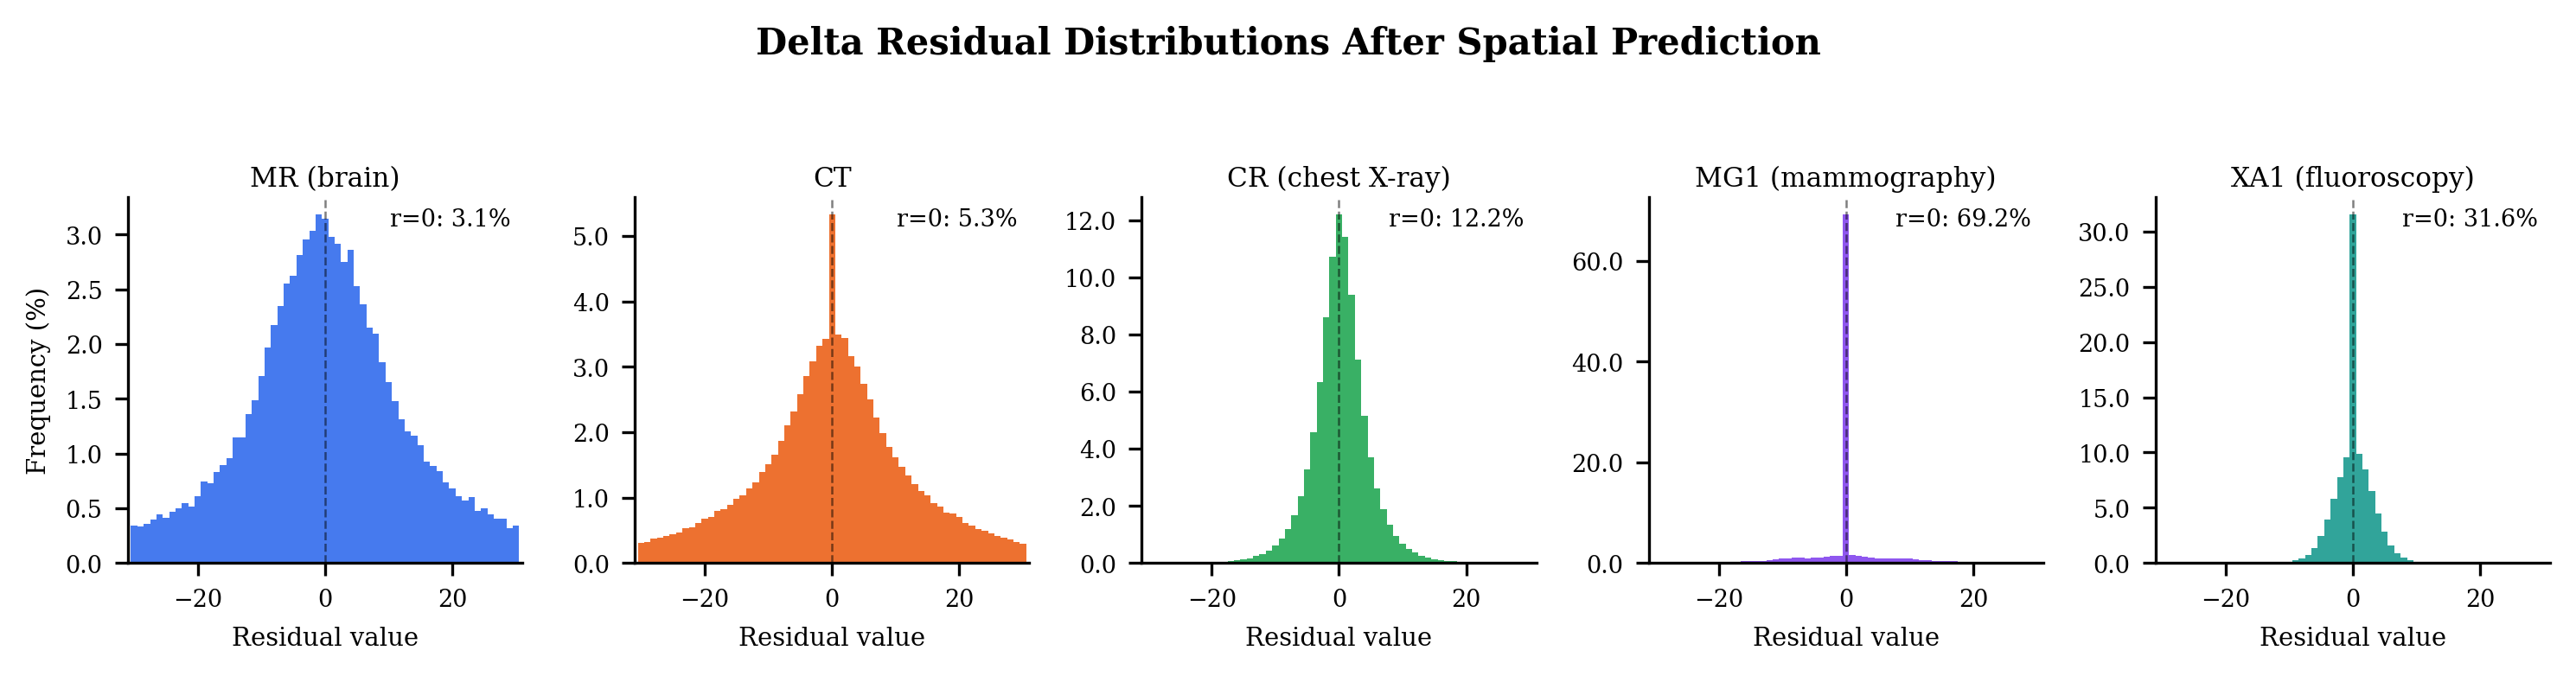
\includegraphics[width=0.85\textwidth]{figures/fig2_histogram.png}
\caption{Delta-residual distributions ($|r| \leq 30$ shown) after avg spatial
prediction. MG1's extreme concentration (69.2\% at zero) explains its
8.79$\times$ compression ratio.}
\label{fig:histogram}
\end{figure*}

\subsection{The Cost-of-Complexity Frontier}

MIC's core Delta+RLE+FSE pipeline achieves a geometric-mean ratio of
3.12$\times$---within 1\% of HTJ2K (3.15$\times$) and 91\% of JPEG-LS
(3.44$\times$)---while decoding faster than both and fitting in roughly
1,100 lines of Go (${\sim}$18$\times$ fewer than HTJ2K's ${\sim}$20k-line
C++ library). JPEG-LS leads on ratio but is the slowest codec evaluated;
HTJ2K has no browser decoder.

\subsection{Lightweight Client-Side Decoding}

A pure JavaScript decoder (${\sim}$20\,KB, zero dependencies) and a Go
WebAssembly build enable client-side in-browser decoding directly from object
storage, eliminating server-side transcoding. Native 16-bit medical image
decoding in the browser requires a purpose-built implementation; MIC provides
one at a fraction of the footprint of general-purpose alternatives.

\subsection{Pathway to Clinical Impact}

MIC could be registered as a DICOM Private Transfer Syntax, allowing PACS
vendors to adopt it without modifying the DICOM standard. The ${\sim}$20\,KB
JavaScript decoder enables a direct storage-and-serve distribution model that
bypasses server-side transcoding entirely.

% ============================================================
\section{Conclusion}
\label{sec:conclusion}

This paper presented MIC, a lossless medical image compression pipeline based on
spatial prediction, 16-bit-native run-length representation, and large-alphabet
table-based entropy coding. The key results across 21 clinical DICOM images
spanning 10 modalities:

\begin{itemize}
  \item \textbf{Compression ratios}: 1.7$\times$--8.9$\times$ across the 21
  evaluated grayscale images.

  \item \textbf{vs.\ Delta+Zstandard}: 5--22\% better compression on all 21
  images (geometric mean $+$14\%), attributable to the structural cost of
  byte-splitting 16-bit residuals.

  \item \textbf{vs.\ HTJ2K}: MIC-4state-C exceeds HTJ2K decompression on 19/21
  images single-threaded (ARM64) and 16/21 (AMD64); PICS-C-8 exceeds HTJ2K on
  all 21 images on both platforms.

  \item \textbf{vs.\ JPEG-LS}: 1.7--5.0$\times$ faster decompression; JPEG-LS
  retains the best lossless ratios (geometric mean 3.44$\times$ vs.\ MIC's
  3.12$\times$).

  \item \textbf{Multi-state decoder}: geometric-mean $+$68\% isolated FSE
  speedup on ARM64 ($+$43\% AMD64) with no ratio penalty.

  \item \textbf{Browser decoder}: ${\sim}$20\,KB pure JS decoder; PICS with
  \texttt{worker\_threads} achieves 483\,MB/s on MG1 in Node.js.

  \item \textbf{Implementation}: approximately 1,100 lines of Go code, about
  18$\times$ fewer source lines than HTJ2K.
\end{itemize}

Overall, the study indicates that 16-bit-native entropy coding is a useful
design point for lossless medical image compression, particularly in
applications where decompression throughput, implementation simplicity, and
deployment portability are important. Future work should strengthen the evidence
base with larger datasets, shuffle-based general-purpose baselines, formal
statistical reporting, and direct browser benchmarking.

MIC is open-source and available at
\url{https://github.com/pappuks/medical-image-codec}.

% ============================================================
\IEEEtriggeratref{35}

\begin{thebibliography}{99}

\bibitem{dicom}
NEMA, ``Digital Imaging and Communications in Medicine (DICOM),''
PS3.5---Data Structures and Encoding, PS3.15---Security and System Management
Profiles,
\url{https://www.dicomstandard.org/}, 2024.

\bibitem{taubman2002}
D.\,S.\,Taubman and M.\,W.\,Marcellin,
\textit{JPEG2000: Image Compression Fundamentals, Standards and Practice}.
Springer, 2002.

\bibitem{htj2k2019}
D.\,S.\,Taubman, ``High throughput JPEG 2000 (HTJ2K): Algorithm, performance
evaluation, and potential,'' \textit{Proc.\ SPIE}, vol.\,11137, 2019.

\bibitem{loco1}
M.\,J.\,Weinberger, G.\,Seroussi, and G.\,Sapiro,
``The LOCO-I lossless image compression algorithm: Principles and
standardization into JPEG-LS,''
\textit{IEEE Trans.\ Image Process.}, vol.\,9, no.\,8, pp.\,1309--1324, 2000.

\bibitem{jpegls2}
ISO/IEC 14495-2:2003, ``Information technology---Lossless and near-lossless
compression of continuous-tone still images: Extensions---Part~2,'' 2003.

\bibitem{jpegxl}
J.\,Alakuijala \textit{et al.},
``JPEG XL next-generation image compression architecture and coding tools,''
\textit{Proc.\ SPIE 11137}, Sep.\,2019.

\bibitem{duda2009}
J.\,Duda, ``Asymmetric numeral systems,'' arXiv:0902.0271, 2009.

\bibitem{duda2013}
J.\,Duda, ``Asymmetric numeral systems: entropy coding combining speed of
Huffman coding with compression rate of arithmetic coding,''
arXiv:1311.2540, 2013.

\bibitem{fse}
Y.\,Collet, ``Finite State Entropy---A new breed of entropy coder,''
\url{https://github.com/Cyan4973/FiniteStateEntropy}, 2013.

\bibitem{rfc8878}
Y.\,Collet and M.\,Kucherawy,
``Zstandard Compression and the `application/zstd' Media Type,''
RFC~8878, IETF, Feb.\,2021.


\bibitem{mahapatra2007}
S.\,Mahapatra and K.\,Singh,
``An FPGA-based implementation of multi-alphabet arithmetic coding,''
\textit{IEEE Trans.\ Circuits Syst.\ I}, vol.\,54, no.\,8, pp.\,1678--1686,
2007.

\bibitem{kosolobov2022}
D.\,Kosolobov, ``Efficiency of ANS Entropy Encoders,''
arXiv:2201.02514, 2022.

\bibitem{bamler2022}
R.\,Bamler, ``Understanding Entropy Coding With Asymmetric Numeral Systems
(ANS): a Statistician's Perspective,'' arXiv:2201.01741, 2022.

\bibitem{giesen2014}
F.\,Giesen, ``Interleaved entropy coders,'' arXiv:1402.3392, 2014.

\bibitem{giesen2014b}
F.\,Giesen, ``ryg\_rans: Public domain rANS encoder/decoder,''
\url{https://github.com/rygorous/ryg_rans}, 2014.

\bibitem{lin2023}
F.\,Lin, K.\,Arunruangsirilert, H.\,Sun, and J.\,Katto,
``Recoil: Parallel rANS Decoding with Decoder-Adaptive Scalability,''
\textit{Proc.\ 52nd ICPP '23}, pp.\,31--40, 2023.

\bibitem{weissenberger2019}
A.\,Weissenberger and B.\,Schmidt,
``Massively Parallel ANS Decoding on GPUs,''
\textit{Proc.\ 48th ICPP '19}, Article~100, 2019.

\bibitem{wu1997}
X.\,Wu and N.\,Memon,
``Context-based, adaptive, lossless image coding,''
\textit{IEEE Trans.\ Commun.}, vol.\,45, no.\,4, pp.\,437--444, 1997.

\bibitem{sneyers2016}
J.\,Sneyers and P.\,Wuille,
``FLIF: Free Lossless Image Format based on MANIAC Compression,''
\textit{Proc.\ IEEE ICIP}, 2016.

\bibitem{legall1988}
D.\,Le Gall and A.\,Tabatabai,
``Sub-band coding of digital images using symmetric short kernel filters and
arithmetic coding techniques,'' \textit{Proc.\ IEEE ICASSP}, pp.\,761--764,
1988.

\bibitem{sweldens1996}
W.\,Sweldens,
``The Lifting Scheme: A custom-design construction of biorthogonal wavelets,''
\textit{Appl.\ Comput.\ Harmon.\ Anal.}, vol.\,3, no.\,2, pp.\,186--200, 1996.

\bibitem{daubechies1998}
I.\,Daubechies and W.\,Sweldens,
``Factoring wavelet transforms into lifting steps,''
\textit{J.\ Fourier Anal.\ Appl.}, vol.\,4, no.\,3, pp.\,247--269, 1998.

\bibitem{calderbank1998}
A.\,R.\,Calderbank, I.\,Daubechies, W.\,Sweldens, and B.-L.\,Yeo,
``Wavelet transforms that map integers to integers,''
\textit{Appl.\ Comput.\ Harmon.\ Anal.}, vol.\,5, no.\,3, pp.\,332--369, 1998.


\bibitem{liu2017}
F.\,Liu \textit{et al.},
``The Current Role of Image Compression Standards in Medical Imaging,''
\textit{Information}, vol.\,8, no.\,4, p.\,131, Oct.\,2017.

\bibitem{clunie2000}
D.\,A.\,Clunie,
``Lossless Compression of Grayscale Medical Images: Effectiveness of
Traditional and State-of-the-Art Approaches,''
\textit{Proc.\ SPIE Medical Imaging}, 2000.

\bibitem{png}
W3C, ``Portable Network Graphics (PNG) Specification (Second Edition),''
ISO/IEC 15948:2003, Nov.\,2003.

\bibitem{taubman2022}
D.\,Taubman, A.\,Naman, M.\,Smith, P.-A.\,Lemieux, H.\,Saadat, O.\,Watanabe,
and R.\,Mathew,
``High Throughput JPEG~2000 for Video Content Production and Delivery Over IP
Networks,''
\textit{Front.\ Signal Process.}, vol.\,2, Article 885644, Apr.\,2022.

\bibitem{williams2009}
S.\,Williams, A.\,Waterman, and D.\,Patterson,
``Roofline: An insightful visual performance model for multicore
architectures,''
\textit{Commun.\ ACM}, vol.\,52, no.\,4, pp.\,65--76, Apr.\,2009.

\bibitem{openjph}
A.\,N.\,Aous,
``OpenJPH: An open-source implementation of High-Throughput JPEG~2000,''
\url{https://github.com/aous72/OpenJPH}, 2024.

\bibitem{charls}
Team CharLS,
``CharLS: A C/C++ JPEG-LS library implementation,''
\url{https://github.com/team-charls/charls}, 2024.


\end{thebibliography}

\end{document}
